\section{Mod\`ele \`a un seul pool de MO}
\subsection{Description du mod\`ele}

\begin{equation}
  {{d[BC]}\over{dt}} =
  \left ( Y_{BC} u_{BC} - kd_{BC} \right ) [BC]
  \label{eq:eq1}
\end{equation}
\begin{equation}
  {{d[TOC]}\over{dt}} =
  -ec [BC]
  \label{eq:eq2}
\end{equation}
\begin{equation}
  {{d[SBC]}\over{dt}} =
  ec [BC] - u_{BC} [BC]
  \label{eq:eq3}
\end{equation}
\begin{equation}
  {{d[SNH_4]}\over{dt}} =
  vNH_4 - nitri
  \label{eq:eq4}
\end{equation}

\par{
Avec
}

\begin{equation}
  ec = e_{1mx} {{[TOC]}\over{k_{1h} + [TOC]}}
  \label{eq:eq5}
\end{equation}
\begin{equation}
  vNH_4 = u_{BC} [BC] (NC)_{TOC} - Y_{BC} u_{BC} [BC] (NC)_{BC}
  \label{eq:eq6}
\end{equation}
\begin{equation}
  nitri = nimax {{[NH_4]}\over{k_{NH_4ni}+[NH_4]}}
  \label{eq:eq7}
\end{equation}

\subsection{Simulation de r\'ef\'erence}

\begin{figure}[h!]
  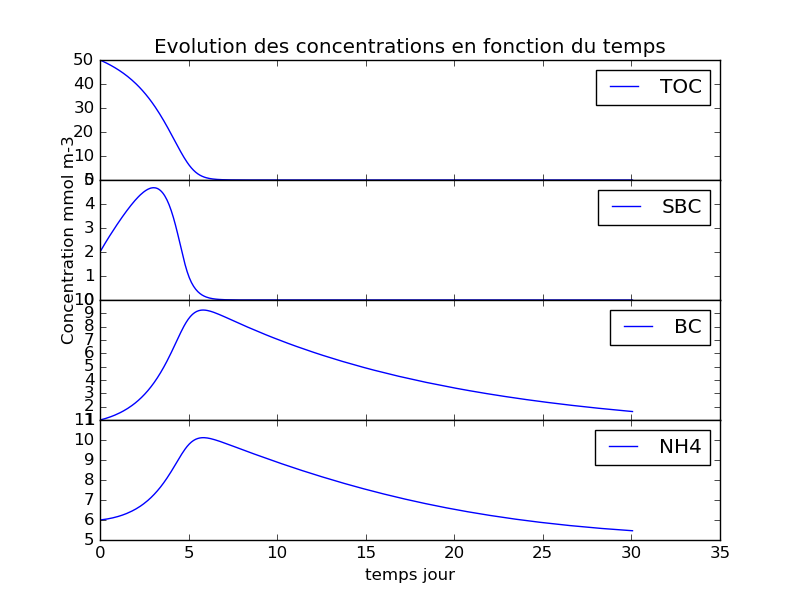
\includegraphics[width=\textwidth]{partie1/Ref.png}
  \caption{Simulation de r\'ef\'erence, pour un mod\`ele \`a un seul pool de mati\`ere organique
  }
  \label{fig:partie1ref}
\end{figure}

\par{
Sur le graphique de l'\'evolution de la concentration du TOC en fonction du temps, nous pouvons observer que la concentration d\'ecro\^it de 0 \`a 6 jours et atteint une valeur nulle apr\`es 6 jours. En effet, ce TOC est hydrolys\'e en SBC, qui d\'epend de la concentration en bact\'eries et de la concentration en TOC. Ainsi, au d\'ebut de la simulation, la d\'ecroissance du TOC est due \`a la grande concentration en TOC (car la valeur de ec est grande). Ensuite, la d\'ecroissance de la concentration de TOC est due \`a une augmentation de la concentration en bact\'eries.
}
\par{
Sur le graphique de l'\'evolution de la concentration en SBC, on peut voir que sa concentration augmente de 0 \`a 4 jours, ou elle atteint une valeur maximale de 4,8 mmolC.m-3, puis d\'ecroit de 4 \`a 6 jours, jusqu'\`a atteindre une valeur nulle. En effet, l'\'evolution de la concentration en SBC est due \`a la concentration en TOC et en SBC. Ainsi, au d\'ebut de la simulation, la concentration en TOC est importante, et celle en SBC est faible, et donc, le terme d'augmentation de la concentration est sup\'erieur au terme de diminution. A 4 jours, les deux termes s'\'egalisent, car la concentration en TOC diminue et car la concentration en SBC augmente. Finalement, apr\`es 4 jours, le terme de diminution de la concentration en SBC diminue jusqu'\`a atteindre une valeur nulle, un peu apr\`es que le TOC atteigne une valeur nulle.
}
\par{
Sur le graphe de l'\'evolution de la concentration en bact\'eries, on peut observer que celle-ci augmente de 0 \`a 6 jours, atteint une valeur maximale de de 9 mmolC.m-3, puis d\'ecro\^it. En effet, l'\'evolution de cette concentration d\'epend de la concentration en SBC. Ainsi, au d\'ebut de la simulation la concentration en SBC augmente, et donc la concentration en bact\'eries augmentent aussi, car le terme de croissance l'emporte sur le terme de mortalit\'e. Au maximum de concentration, les deux termes se compensent, car la concentration en SBC diminue. Finalement, la concentration en SBC devient nulle, et donc seul le terme de mortalit\'e influence l'\'evolution de la concentration en bact\'eries.
}
\par{
Sur le graphe de l'\'evolution de la concentration en NH4, celle-ci augmente de 0 \`a 6 jours, pour atteindre un maximum de 10 mmolC.m-3, puis d\'ecro\^itre ensuite. En effet, l'\'evolution de la concentration d\'epend de deux termes: une terme d\'ependant de ce qu'utilise les bact\'eries, par rapport \`a ce dont elles ont besoins (vNH4, d\'ependant de la concentration en bact\'eries et de la concentration en SBC), et un terme de nitrification, d\'ependant de la concentration en NH4. Au d\'ebut de la simulation, la concentration en NH4 augmente, ce qui veut dire que la valeur de vNH4 est sup\'erieur au terme de nitrification. Ainsi, le terme vNH4 est toujours positif, ce qui signifie que ce qu'utilisent les bact\'eries est toujours sup\'erieur \`a ce qu'elles ont besoin, et donc qu'elles rejettent du NH4 dans leur environnement. Au maximum de concentration en NH4, les deux termes se compensent, car la concentration en SBC diminue. Finalement, lorsque la concentration en SBC devient nulle, l'\'evolution de NH4 ne d\'epend plus que de la nitrification.
}

\subsection{Tests de sensitivit\'e}
\subsubsection{Test 1}

\begin{figure}[h!]
  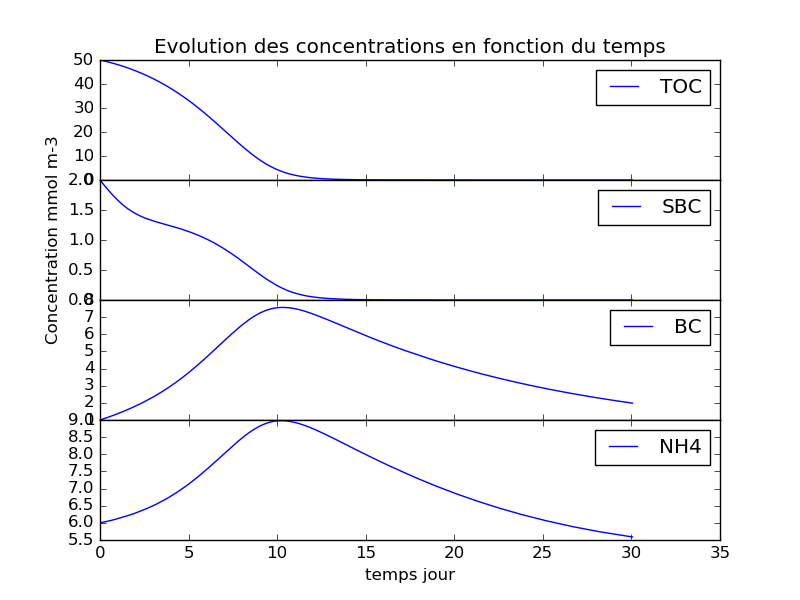
\includegraphics[width=\textwidth]{partie1/Test1.png}
  \caption{Simulation en divisant par deux la valeur de la constante d'ectohydrolyse de TOC \`a temp\'erature optimale
  }
  \label{fig:partie1test1}
\end{figure}



\subsubsection{Test 2}

\begin{figure}[h!]
  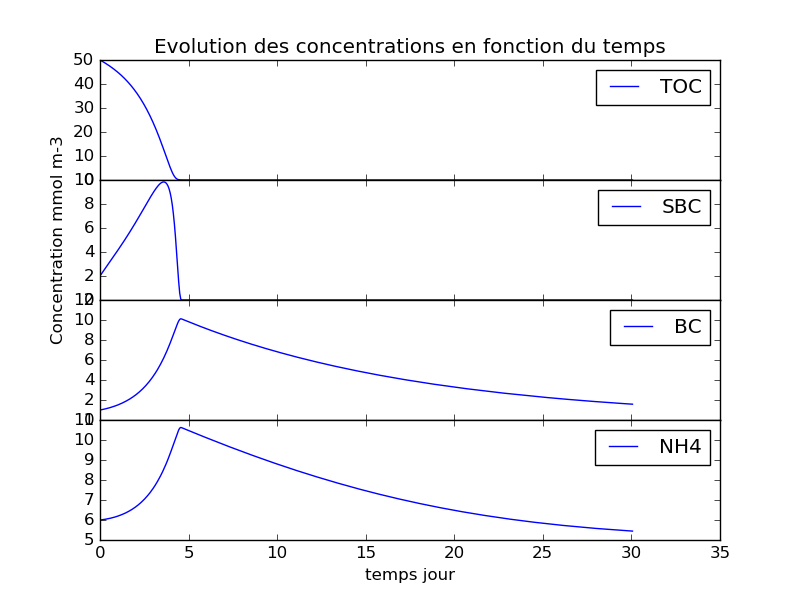
\includegraphics[width=\textwidth]{partie1/Test2.png}
  \caption{Simulation en r\'eduisant la valeur de la constante d'hydrolyse de TOC
  }
  \label{fig:partie1test2}
\end{figure}

\subsubsection{Test 3}

\begin{figure}[h!]
  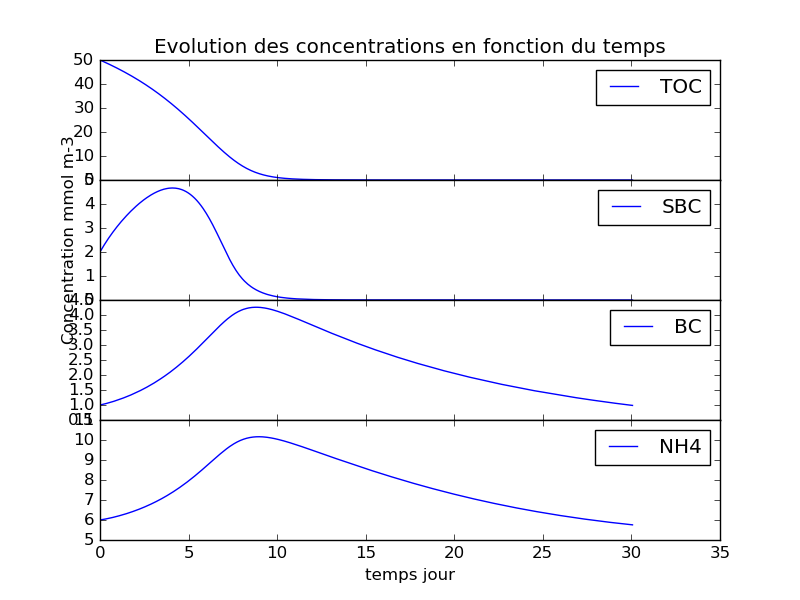
\includegraphics[width=\textwidth]{partie1/Test3.png}
  \caption{Simulation en r\'eduisant la valeur du taux de croissance des bact\'eries
  }
  \label{fig:partie1test3}
\end{figure}

\subsubsection{Test 4}

\begin{figure}[h!]
  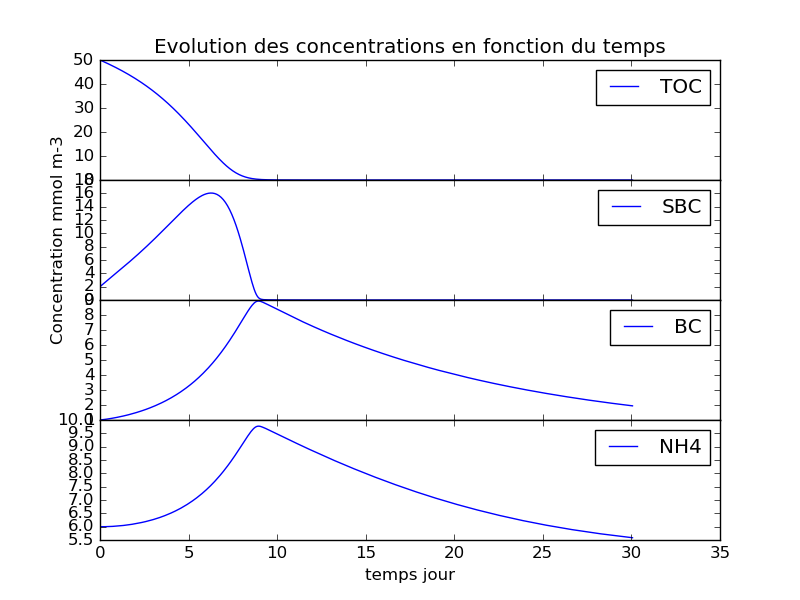
\includegraphics[width=\textwidth]{partie1/Test4.png}
  \caption{Simulation en r\'eduisant la valeur de la constante d'uptake de SBC \`a temp\'erature optimale
  }
  \label{fig:partie1test4}
\end{figure}

\subsubsection{Test 5}


\begin{figure}[h!]
  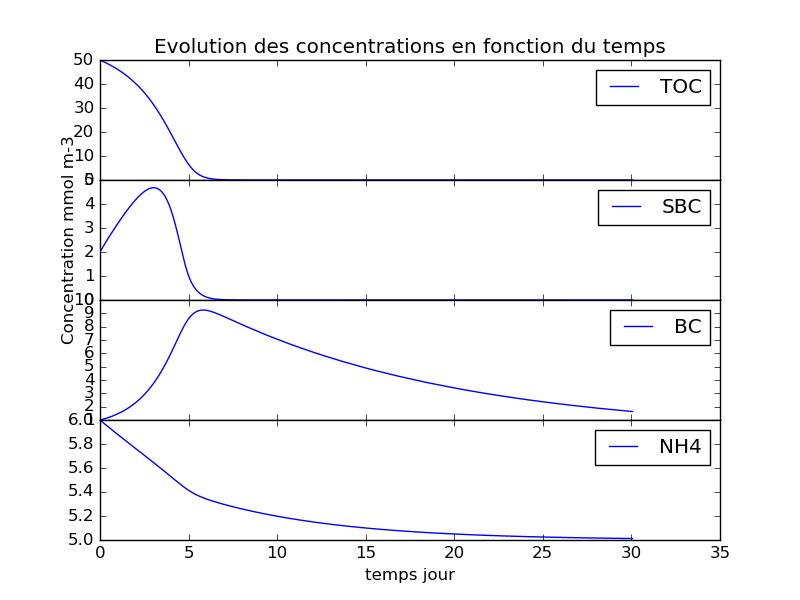
\includegraphics[width=\textwidth]{partie1/Test5.png}
  \caption{Simulation en r\'eduisant la valeur du rapport NC du TOC
  }
  \label{fig:partie1test5}
\end{figure}

\subsubsection{Test 6}

\begin{figure}[h!]
  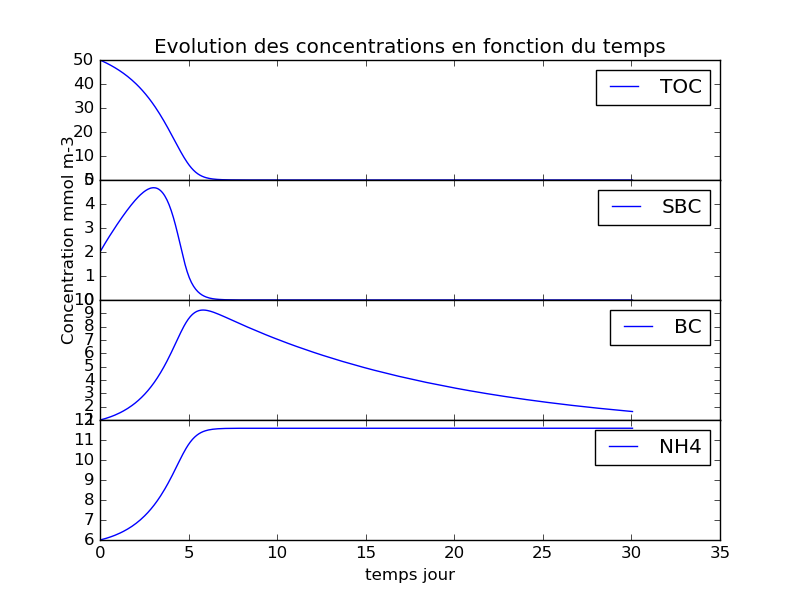
\includegraphics[width=\textwidth]{partie1/Test6.png}
  \caption{Simulation en supprimant l'effet de la nitrification
  }
  \label{fig:partie1test6}
\end{figure}

\subsection{Conclusion}